\section{Μοντελοποίηση Κινητήρων}
\noindent Η μοντελοποίηση των κινητήρων είναι σημαντική για την εφαρμογή του 
ελεγκτή στον μικροελεγκτή \tl{PIXHAWK}. Ως σήμα δράσης, χρησιμοποιούνται οι 
τάσεις εισόδου του κάθε κινητήρα κινητήρα. Απαιτείται, λοιπόν, η σύνδεση τους με
τις αντίστοιχες γωνιακές ταχύτητες των κινητήρων, οι οποίες αποτελούν μεταβλητές 
δράσης για τον ελεγκτή. 

Οι δύο εμπρόσθιοι κινητήρες, που είναι συνδεδεμένοι στο αερόχημα, 
είναι οι \tl{AXI 2200/12 V2 Long Gold Line}, ενώ επιλέχθηκε ως οπίσθιος 
κινητήρας ο \tl{AXI 2826/10 Gold Line}. Οι συγκεκριμένοι κινητήρες είναι 
ηλεκτρικοί κινητήρες συνεχούς ρεύματος χωρίς ψήκτρες \tl{(BLDC)}.

\begin{figure}[hbt!]
    \begin{subfigure}{0.48\textwidth}
        \centering
        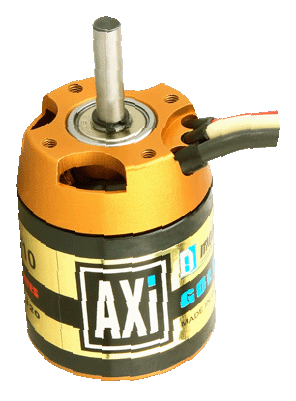
\includegraphics[scale=0.3]{Motor/AXI2826_10_GL_1.png} 
        \caption{\tl{AXI 2826/10 Gold Line}}
        \label{AXI2826}
    \end{subfigure}
    \begin{subfigure}{0.48\textwidth}
        \centering
        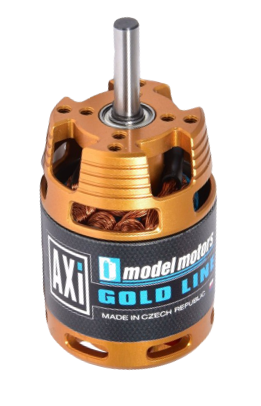
\includegraphics[scale=0.3]{Motor/AXI2220_12_v2_long_1.png}
        \caption{\tl{AXI 2200/10 V2 Long Gold Line}}
        \label{AXI2200}
    \end{subfigure}
    \caption{\tl{BLDC} Κινητήρες}
    \label{fig:image2}
\end{figure}

Το ισοδύναμο μοντέλο τέτοιου είδους κινητήρων φαίνεται στο σχήμα 
(\ref{circuit}). Περιλαμβάνει την πηγή τάσης  \(v\), μία ισοδύναμη αντίσταση 
\(R\) και επαγωγή \(L\) και την τάση \(v_m\), που αναπτύσσεται στο εσωτερικό του 
κινητήρα. 

\begin{figure}[hbt!]
    \centering
    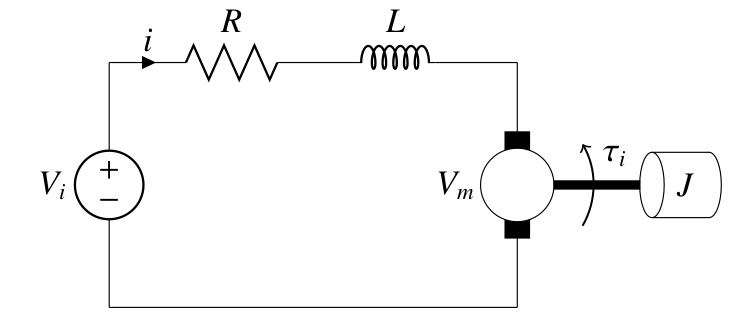
\includegraphics[scale=0.3]{Motor/Electric_Circuit.png}
    \caption{Ηλεκτρονικό Κύκλωμα Κινητήρα}\label{circuit}
\end{figure}

Εφαρμόζεται στο ηλεκτρικό κύκλωμα ο νόμος της τάσης του \tl{Kirchoff} και 
προκύπτει

\begin{equation*}
    v - R i - L\frac{di}{dt} - v_m = 0.
\end{equation*}

Η συνεισφορά του επαγωγικού όρου θεωρείται αμελητέα, εφόσον τα δυναμικά 
χαρακτηριστικά της ηλεκτρικής συνιστώσας είναι αρκετά ταχύτερα από αυτά της
μηχανικής. Επομένως

\begin{equation}
    v - R i - v_m = 0.
    \label{mtr:Kirchoff}
\end{equation}

Οι συγκεκριμένοι κινητήρες επιπλέον χαρακτηρίζονται από την γραμμική σχέση 
ανάμεσα στην περιστροφική ταχύτητα και την εσωτερική τάση, καθώς και ανάμεσα 
στην ροπή και το ρεύμα του κυκλώματος. Οι σχέσεις αυτές είναι
\begin{gather*}
    \omega = K_v v_m\\
    Q = K_t (i - i_0)
\end{gather*}
\begin{conditions}
    K_v & χαρακτηριστική σταθερά του κινητήρα $(\frac{rad/s}{v})$\\
    K_t & χαρακτηριστική σταθερά του κινητήρα $(\frac{v}{rad/s})$\\
    i_0 & σταθερό ρεύμα κινητήρα χωρίς φορτίο (σταθερά του κινητήρα).
\end{conditions}

Αντικαθιστώντας τις γραμμικές σχέσεις στον νόμο τάσης του \tl{Kirchoff}, 
συντίθεται η σχέση
\begin{equation*}
    v = K_v \omega + \frac{Q R}{K_t} + i_0 R.
\end{equation*}

Ωστόσο, στην μοντελοποίηση των ελίκων, ορίστηκε τετραγωνική σχέση της ροπής
με την γωνιακή ταχύτητα. Στη μόνιμη κατάσταση, η ροπή, που προσδίδει ο 
κινητήρας, είναι ίση με την ροπή αντίστασης της έλικας \(Q = N = \beta 
\omega^2\). Έτσι η παραπάνω σχέση γίνεται
\begin{equation*}
    v = K_v \omega + \frac{\beta R}{K_t}\omega^2 + i_0 R.
\end{equation*}

Οι σταθερές \(K_v, K_t, R, i_0\) αποτελούν κατασκευαστικά χαρακτηριστικά του
κινητήρα και δίνονται από τον κατασκευαστή. Επιπλέον ισχύει 
$K_v = \frac{1}{K_t}$.